\section{Beschreibung grundlegender Klassen}
Alle Klassen wurden in folgende Packages unterteilt. Im folgenden werden diese vom Gesamtprogram isoliert betrachtet. Eine globale "Ubersicht "uber s"amtliche Zusammenh"ange findet sich erst im Kapitel ...
\todo{Kapitelref einfuegen}
\begin{itemize}
	\item \ref{ss:token} \nameref{ss:token}
	\begin{itemize}
		\item \nameref{par:pos}
		\item \nameref{par:districtType}
		\item \nameref{par:tiles}
		\item \nameref{par:singleTile}
		\item \nameref{par:domino}
	\end{itemize}
\end{itemize}

\newpage
\subsection{token}
\label{ss:token}
Das package \emph{token} (siehe Abbildung \ref{fig:tokenPackage}) vereint s"amtliche Klassen die ben"otigt werden um einen Domino (siehe \nameref{par:domino}) erstellen zu k"onnen. 

\begin{figure}
	\centering
	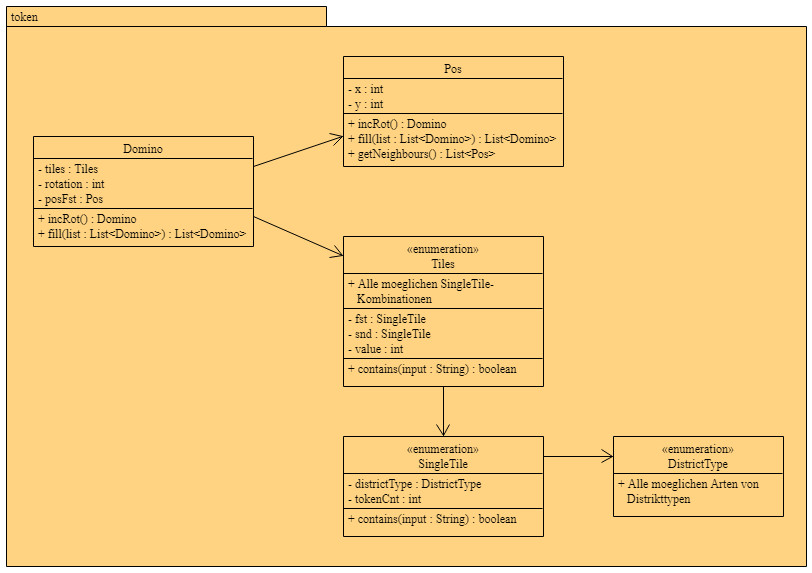
\includegraphics{pics/tokenPackage}
	\caption{UML-Darstellung des token packages}
	\label{fig:tokenPackage}
\end{figure}

\paragraph{Pos}
\label{par:pos}
Diese Klasse wurde von der Bonusaufgabe der PS2-"Ubungung "ubernommen. Es wurde lediglich \emph{toString()}-Methode sowie \emph{getNeighbours()} abge"andert und einige Konstanten hinzugef"ugt um den Checkstyle-Richtilinien 
(siehe Abschnitt \ref{sec:entwicklungskonfiguration} - \nameref{sec:entwicklungskonfiguration}) 
folge zu leisten. Dennoch folgt hier ein kurzer "Uberblick "uber diese Klasse: 

Eine Position setzt sich aus einer x- und einer y-Komponente zusammen. Diese sind als \emph{final} deklariert und k"onnen somit nicht ver"andert werden. Neben dem Konstruktor und diversen Gettern gibt es eine Methode um festzustellen ob sich eine gegebene Position neben der Position des Objekts befindet. Dazu wird ein die Differenz der beiden jeweils gleichnamigen Komponenten gebildet und am Ende verglichen ob nur jeweils eine der beiden Differenzen gleich Null ist. 

\begin{lstlisting}[style=CodeHighlighting]
public boolean isNextTo(Pos p) {
    int xDiff = Math.abs(x - p.x());
	int yDiff = Math.abs(y - p.y());
	return (xDiff == 1 && yDiff == 0
            || xDiff == 0 && yDiff == 1);
}
\end{lstlisting}

Die Methode \emph{getNeighbours()} liefert eine Arraylist der vier Nachbarn. Hierzu wird eine Liste initialisiert und mit neuen Positionen bef"ullt deren x- und y-Komponenten entsprechend modifiziert werden. 

\begin{lstlisting}[style=CodeHighlighting]
public List<Pos> getNeighbours() {
    List<Pos> neighbours = new ArrayList<>();
    neighbours.add(LEFT_ROT, new Pos(this.x - 1, this.y));
    neighbours.add(DOWN_ROT, new Pos(this.x, this.y - 1));
    neighbours.add(RIGHT_ROT, new Pos(this.x + 1, this.y));
    neighbours.add(UP_ROT, new Pos(this.x, this.y + 1));
    return neighbours;
}
\end{lstlisting}


Eine \emph{equals}-Methode ist auch implementiert, diese vergleicht allerdings nur die jeweiligen x- und y-Komponenten der beiden Positionen. Bei der \emph{toString}-Methode ist ein werden die beiden Komponten zwischen einem Klammernpaar und mit Komma getrennt ausgegeben. 

\paragraph{DistrictType}
\label{par:districtType}
In diesem Aufz"ahlungstyp werden die m"oglichen Kategorien der Distrikte aufgef"uhrt. Wichtig hierbei, auch ein leeres Feld sowie das Stadtzentrum besitzen einen Typ. 
Dieser Aufz"ahlungstyp spielt vor allem beim Ausz"ahlen der Punkte beziehungsweise dem verwalten der verschiedenen Distrikte eine wichtige Rolle. 

\begin{lstlisting}[style=CodeHighlighting]
public enum DistrictType {
    EMPTY_CELL, CENTER, AMUSEMENT, INDUSTRY, OFFICE, PARK, SHOPPING, HOME
}
\end{lstlisting}


\paragraph{SingleTile}
\label{par:singleTile}
Dieser Aufz"ahlungstyp repr"asentiert einen Domino Aufdruck. 

Ein Konstruktur verbindet die Enum-Darstellung mit einem Distrikttypen und einem Anzahl an Punkten welche auf dem betrachteten Tile verf"ugbar sind. 

\begin{lstlisting}[style=CodeHighlighting]
CC(CENTER, 0), EC(EMPTY_CELL, 0),
A0(AMUSEMENT, 0), A1(AMUSEMENT, 1), A2(AMUSEMENT, 2), A3(AMUSEMENT, 3),
I0(INDUSTRY, 0), I1(INDUSTRY, 1), I2(INDUSTRY, 2), I3(INDUSTRY, 3),
O0(OFFICE, 0), O1(OFFICE, 1), O2(OFFICE, 2), O3(OFFICE, 3),
P0(PARK, 0), P1(PARK, 1), P2(PARK, 2), P3(PARK, 3),
S0(SHOPPING, 0), S1(SHOPPING, 1), S2(SHOPPING, 2), S3(SHOPPING, 3),
H0(HOME, 0), H1(HOME, 1), H2(HOME, 2), H3(HOME, 3);

private DistrictType districtType;

private int tokenCnt;

SingleTile(DistrictType disctrictType, int tokenCnt) {
    this.districtType = disctrictType;
    this.tokenCnt = tokenCnt;
}
\end{lstlisting}

Au"serdem verf"ugt der Aufz"ahlungstyp "uber Getter f"ur beide Felder und eine Methode die "uberpr"uft ob eine gegebene String repr"asentation einer dem Wert eines der Enumobjekte entspricht. Hierzu wird eine Schleife durchlaufen die beim Fund mit \emph{true} und ansonsten mit \emph{false} abbricht. 

\paragraph{Tiles}
\label{par:tiles}
Dieser Aufz"ahlungstyp beschreibt alle m"oglichen \emph{SingleTile}-Kombinationen die im Stapel einer normalen Partie des Spiels m"oglich sind. 

\begin{lstlisting}[style=CodeHighlighting]
P0P0_Val1(P0, P0, 1),
P0P0_Val2(P0, P0, 2),
...
O0I2_Val47(O0, I2, 47),
P0I3_Val48(P0, I3, 48);

public static final int TILES_CNT = Tiles.values().length;

private final SingleTile fst;
private final SingleTile snd;

private final int value;

Tiles(SingleTile fst, SingleTile snd, int value) {
    this.fst = fst;
    this.snd = snd;
    this.value = value;
}
\end{lstlisting}

Auch hier gibt es wieder einen Konstruktor der diverse Werte an die jeweiligen Enum-Werte bindet. Es werden neben den beiden SingleTile-Kombinationen auch der Wert dieser spezifischen Kombination gespeichert. Der Wert dient dem Sortieren der B"anke und wurde aus der Aufgabenstellung entnommen (wurde also nicht willk"urliche festgelegt). 

Um einfacher Testen zu k"onnen wurden mehrere Methoden eingef"uhrt um von au"serhalb einfacher bestimmte Tile-Kombinationen zu bekommen. Diese sind allerdings im Hauptprogramm nicht von Bedeutung. Neben sonstigen Gettern besitzt diese Klasse lediglich eine \emph{toString()}-Methode wo nur die ersten 4 Buchstaben der Enum-Werte zur"uckgegeben werden, da diese die Tile-Kombination angeben, der Wert der Kombination entf"allt hierbei (ist aber in dieser Methode auch unbedeutend).

Um eine gegebene Liste zu f"ullen wird die Methode \emph{fill} bereitgestellt. Hierbei wird eine gegebene Liste geleert und mit allen m"oglichen unterschiedlichen Dominos gef"ullt. 

\begin{lstlisting}[style=CodeHighlighting]
public static List<Domino> fill(List<Domino> list) {
    if (null == list) {
        list = new LinkedList<>();
    } else {
        list.clear();
    }
    for (Tiles tile : Tiles.values()) {
        list.add(new Domino(tile, DEFAULT_POS));
    }
    return list;
}
\end{lstlisting}

\paragraph{Domino}
\label{par:domino}
Diese Klasse vereint s"amtliche zuvor genannten Datenstrukturen. 

Ein Domino besitzt eine bestimmte Kombination aus SingleTiles und eine Rotation sowie Position. Letztere beiden beziehen sich auf ein Board, nicht auf eine Bank oder dergleichen. 